\renewcommand*{\arraystretch}{1.1}

\subsection*{BI / read / 18}
\label{section:bi-read-18}

% change \emph{} to use sans-serif font
\let\oldemph\emph
\renewcommand{\emph}[1]{{\footnotesize \sf #1}}

\renewcommand{\currentQueryCard}{18}
\marginpar{
	\raggedleft
	\vspace{0.22ex}

    \queryRefCard{bi-read-01}{BI}{1}\\
    \queryRefCard{bi-read-02}{BI}{2}\\
    \queryRefCard{bi-read-03}{BI}{3}\\
    \queryRefCard{bi-read-04}{BI}{4}\\
    \queryRefCard{bi-read-05}{BI}{5}\\
    \queryRefCard{bi-read-06}{BI}{6}\\
    \queryRefCard{bi-read-07}{BI}{7}\\
    \queryRefCard{bi-read-08}{BI}{8}\\
    \queryRefCard{bi-read-09}{BI}{9}\\
    \queryRefCard{bi-read-10}{BI}{10}\\
    \queryRefCard{bi-read-11}{BI}{11}\\
    \queryRefCard{bi-read-12}{BI}{12}\\
    \queryRefCard{bi-read-13}{BI}{13}\\
    \queryRefCard{bi-read-14}{BI}{14}\\
    \queryRefCard{bi-read-15}{BI}{15}\\
    \queryRefCard{bi-read-16}{BI}{16}\\
    \queryRefCard{bi-read-17}{BI}{17}\\
    \queryRefCard{bi-read-18}{BI}{18}\\
    \queryRefCard{bi-read-19}{BI}{19}\\
    \queryRefCard{bi-read-20}{BI}{20}\\
    \queryRefCard{bi-read-21}{BI}{21}\\
    \queryRefCard{bi-read-22}{BI}{22}\\
    \queryRefCard{bi-read-23}{BI}{23}\\
    \queryRefCard{bi-read-24}{BI}{24}\\
    \queryRefCard{bi-read-25}{BI}{25}\\
}


\noindent\begin{tabularx}{\queryCardWidth}{|>{\queryPropertyCell}p{\queryPropertyCellWidth}|X|}
	\hline
	query & BI / read / 18 \\ \hline
%
	title & How many persons have a given number of messages
 \\ \hline
%
	pattern & \hfill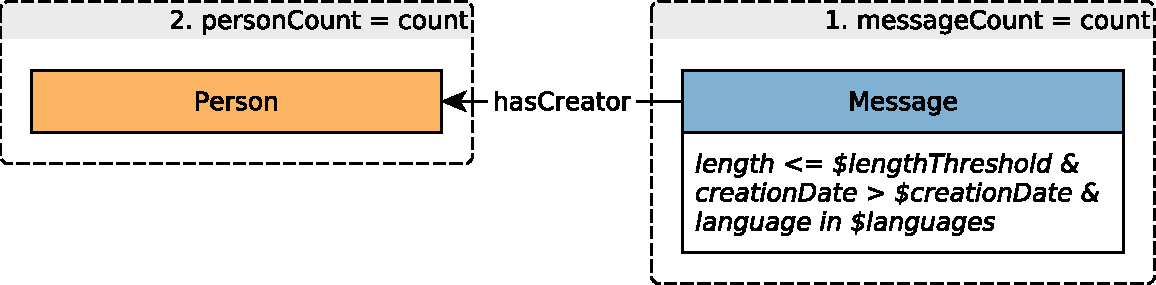
\includegraphics[scale=\patternscale,margin=0cm .2cm]{patterns/bi-read-18}\hfill\vadjust{} \\ \hline
%
	desc. & For each \emph{Person}, count the number of \emph{Messages} they made
(\texttt{messageCount}). Only consider \emph{Messages} with the
following attributes:

\begin{itemize}
\item
  \texttt{content} not empty (and consequently, \texttt{imageFile} empty
  for \emph{Posts}),
\item
  \texttt{length} below the \texttt{lengthThreshold} (exclusive,
  equality is not allowed),
\item
  \texttt{creationDate} after \texttt{date} (exclusive, equality is not
  allowed),
\item
  The \emph{Message} is written in any of the given \texttt{languages}.
\item
  The language of a \emph{Post} is defined by its \texttt{language}
  attribute.
\item
  The language of a \emph{Comment} is that of the \emph{Post} that
  initiates the thread where \emph{Comment} replies to.
\end{itemize}

For each \texttt{messageCount} value, count the number of \emph{Persons}
with exactly \texttt{messageCount} \emph{Messages} (with the required
attributes).
 \\ \hline
%
	
		params &
		\innerCardVSpace{\begin{tabularx}{\attributeCardWidth}{|>{\paramNumberCell}c|>{\varNameCell}M|>{\typeCell}m{\typeWidth}|Y|} \hline
		$\mathsf{1}$ & date
 & Date
 &  \\ \hline
		$\mathsf{2}$ & lengthThreshold
 & 32-bit Integer
 &  \\ \hline
		$\mathsf{3}$ & languages
 & String{[}{]}
 &  \\ \hline
		\end{tabularx}}\innerCardVSpace \\ \hline
	
%
	
		result &
		\innerCardVSpace{\begin{tabularx}{\attributeCardWidth}{|>{\resultNumberCell}c|>{\varNameCell}M|>{\typeCell}m{\typeWidth}|>{\resultOriginCell}c|Y|} \hline
		$\mathsf{1}$ & messageCount & 32-bit Integer & A &
				Number of \emph{Messages} created
 \\ \hline
		$\mathsf{2}$ & personCount & 32-bit Integer & A &
				The number of \emph{Persons} with \texttt{messageCount} messages
 \\ \hline
		\end{tabularx}}\innerCardVSpace \\ \hline
	
%
	
		sort		&
		\innerCardVSpace{\begin{tabularx}{\attributeCardWidth}{|>{\sortNumberCell}c|>{\varNameCell}M|>{\directionCell}c|Y|} \hline
		$\mathsf{1}$ & personCount
 & $\desc
$ &  \\ \hline
		$\mathsf{2}$ & messageCount
 & $\desc
$ &  \\ \hline
		\end{tabularx}}\innerCardVSpace \\ \hline
	%
	%
	CPs &
	\multicolumn{1}{>{\raggedright}l|}{
		\chokePoint{1.1}, 
		\chokePoint{1.2}, 
		\chokePoint{1.6}, 
		\chokePoint{3.2}, 
		\chokePoint{4.2}, 
		\chokePoint{4.3}
		} \\ \hline
	%
	%
\end{tabularx}
\queryCardVSpace

% change \emph back to the old one
\renewcommand{\emph}[1]{\oldemph{#1}}